% !TeX encoding = UTF-8

\documentclass{protokol}

\usepackage{pdfpages}
\usepackage{tikz}
\usetikzlibrary{calc}
\usetikzlibrary{arrows}

%====== Units =====
\usepackage{siunitx}
\sisetup{inter-unit-product =\ensuremath{\cdot}}
\sisetup{group-digits = integer}
\sisetup{output-decimal-marker = {,}}
\sisetup{exponent-product = \ensuremath{\cdot}}
\sisetup{separate-uncertainty}
\sisetup{tight-spacing = false}
%\sisetup{scientific-notation = true}
%\sisetup{round-mode=places,round-precision=4}
%\sisetup{evaluate-expression}


%====== Grafy =====
\usepackage{pgfplots}
\pgfplotsset{width=0.8\linewidth, compat=1.17}
\def\plotcscale{0.8}
\usepackage{pgfplotstable}
\usepackage[figurename=Obr.]{caption} % figure caption rename

%====== Rovnice align block ======
\usepackage{amsmath}
\setlength{\jot}{10pt} % rozestup mezi řádky

\graphicspath{ {./img/} }

%====== Vyplňte údaje ======
\jmeno{Jakub Charvot}
\kod{240844}
\rocnik{3.}
\obor{MET}
\skupina{MET/2}
\spolupracoval{Radek Kučera}

\merenodne{12.03.\ 2024}
\odevzdanodne{19.03.\ 2024}
\nazev{Měření atmosférického tlaku}
\cislo{4} %měřené úlohy

\predmet{Mikrosenzory a mikromechanické systémy}
\ustav{Ústav mikroelektroniky}
\skola{FEKT VUT v~Brně}

\def\para{x+0}
\def\parb{\para-80}


% %citace 
% \usepackage[backend=biber, style=iso-numeric, sortlocale=cs_CZ, autolang=other, language=czech]{biblatex}
% \addbibresource{bibliography.bib}
% \DeclareFieldFormat{labelnumberwidth}{\mkbibbrackets{#1}}
% hyperlinky
\usepackage[colorlinks]{hyperref}

% odstavce
\usepackage{parskip}

% Bloky kódu
\usepackage{xcolor}

%New colors defined below
\definecolor{codegreen}{rgb}{0,0.6,0}
\definecolor{codegray}{rgb}{0.5,0.5,0.5}
\definecolor{codepurple}{rgb}{0.58,0,0.82}
\definecolor{backcolour}{rgb}{0.95,0.95,0.92}

\usepackage{listings}
\lstdefinestyle{mystyle}{
  backgroundcolor=\color{backcolour}, commentstyle=\color{codegreen},
  keywordstyle=\color{magenta},
  numberstyle=\tiny\color{codegray},
  stringstyle=\color{codepurple},
  basicstyle=\ttfamily\footnotesize,
  breakatwhitespace=false,         
  breaklines=true,                 
  captionpos=b,                    
  keepspaces=true,                 
  numbers=left,                    
  numbersep=5pt,                  
  showspaces=false,                
  showstringspaces=false,
  showtabs=false,                  
  tabsize=2
}
\lstset{
	inputencoding=utf8,
	extendedchars=true,
	literate={á}{{\'a}}1 {č}{{\v{c}}}1 {ď}{{\v{d}}}1 {é}{{\'e}}1 {ě}{{\v{e}}}1 
           {í}{{\'i}}1 {ň}{{\v{n}}}1 {ó}{{\'o}}1 {ř}{{\v{r}}}1 {š}{{\v{s}}}1 
           {ť}{{\v{t}}}1 {ú}{{\'u}}1 {ů}{{\r{u}}}1 {ý}{{\'y}}1 {ž}{{\v{z}}}1 
           {Á}{{\'A}}1 {Č}{{\v{C}}}1 {Ď}{{\v{D}}}1 {É}{{\'E}}1 {Ě}{{\v{E}}}1 
           {Í}{{\'I}}1 {Ň}{{\v{N}}}1 {Ó}{{\'O}}1 {Ř}{{\v{R}}}1 {Š}{{\v{S}}}1 
           {Ť}{{\v{T}}}1 {Ú}{{\'U}}1 {Ů}{{\r{U}}}1 {Ý}{{\'Y}}1 {Ž}{{\v{Z}}}1,
	style=mystyle
	}

% Číslování
\pagenumbering{arabic}

% Tabulky
\usepackage{booktabs}

% =========================================
% =============== DOKUMENT ================
% =========================================
\begin{document}
	%====== Vygenerování tabulky ======a
    \maketitle

    \section{Měření a jeho vyhodnocení }
        Nejprve jsme měřícím přístrojem (ALMEMO) stanovili možný rozsah měření. V komoře lze dosáhnout tlaků v rozmezí \num{625,5} až \qty{948,6}{\milli\bar}. 

    \begin{table}[ht!]
        \caption{Měřené (\(p_{ref}, U_{out}  \)) a vypočtené hodnoty.}
        \def\arraystretch{1.2}
        \centering
        \begin{tabular}{rrrrr}
\toprule
$\theta_{rot-nast}\ [^\circ]$ & $\theta_{rot-mer}\ [^\circ]$ & $\Delta \theta_{rot} \ [^\circ]$ & $\theta_{nak-nast}\ [^\circ]$ & $\theta_{nak-mer}\ [^\circ]$ \\
\midrule
90,000 & 87,138 & 2,047 & 90,000 & 87,953 \\
80,000 & 77,793 & 1,171 & 80,000 & 78,829 \\
70,000 & 67,770 & 0,715 & 70,000 & 69,285 \\
60,000 & 57,801 & 0,563 & 60,000 & 59,437 \\
50,000 & 48,346 & 0,184 & 50,000 & 49,816 \\
40,000 & 38,345 & 0,037 & 40,000 & 39,963 \\
30,000 & 28,879 & -0,346 & 30,000 & 30,346 \\
20,000 & 18,929 & 0,019 & 20,000 & 19,981 \\
10,000 & 9,645 & -1,123 & 10,000 & 11,123 \\
0,000 & -0,448 & -1,560 & 0,000 & 1,560 \\
-10,000 & -11,354 & -0,831 & -10,000 & -9,169 \\
-20,000 & -21,389 & -0,575 & -20,000 & -19,425 \\
-30,000 & -30,961 & -0,509 & -30,000 & -29,491 \\
-40,000 & -39,973 & -1,043 & -40,000 & -38,957 \\
-50,000 & -50,243 & -0,828 & -50,000 & -49,172 \\
-60,000 & -59,785 & -1,243 & -60,000 & -58,757 \\
-70,000 & -70,255 & -1,390 & -70,000 & -68,610 \\
-80,000 & -79,226 & -1,078 & -80,000 & -78,922 \\
-90,000 & -88,276 & -1,904 & -90,000 & -88,096 \\
\bottomrule
\end{tabular}

    \end{table}

    \subsection{Příklad výpočtu}
        Hodnoty z přístroje ALMEMO převedeme na kPa. 

        % # Calculate MPX4115A pressure (kPa) according to datasheet
        % # Datasheet transfer function:
        % # V_out = V_S * (P*0.009 - 0.095) +- (Pressure Error * Temp Error * 0.009 * V_S)
        % # V_out = V_S * ((P*0.009 - 0.095) +- (Pressure Error * Temp Error * 0.009))
        % # V_out = V_S * (0.009(P+- (Pressure Error * Temp Error)) - 0.095)
        % # V_out / V_S + 0.095 = 0.009(P+- (Pressure Error * Temp Error))
        % # P +- (Pressure Error * Temp Error) = (V_out / V_S + 0.095) / 0.009
        Vyjdeme ze vztahu z katalogového listu senzoru MPX4115A:
        \[
            U_{out} = V_{S} \cdot (p_{out}\cdot \num{0.009}-\num{0.095})\pm (PressureError \cdot TempErrorFactor\cdot \num{0.009}\cdot V_{S} ) 
        \]
        Pro běžné teploty platí \(TempErrorFactor=1\). Pro námi měřené tlaky pak platí \(PressureError(max)=\qty{1.5}{\kilo\pascal}\) 
        
        Jednoduchou úpravou získáme vztah:
        \[
            p_{out} = \frac{\frac{U_{out}}{V_{S}}+\num{0.095}}{0.009} \pm PressureError
        \]
        Po dosazení prvního řádku tabulky vychází:
        \[
            p_{out} = \frac{\frac{\num{3.657}}{5}+\num{0.095}}{0.009} \pm \num{1.5}
        \]
        \[
            p_{out} = \qty{91.8+-1.5}{kPa}
        \]

        Výpočet chyb měření:
        \begin{align*}
            \Delta_{p} =& p_{out} - p_{ref}  \\
            \Delta_{p} =& \num{91.822} - \num{94.86}  \\
            \Delta_{p} =& \qty{-3,038}{kPa}
        \end{align*}

        \begin{align*}
            \delta_{p} =& \frac{\Delta_{p}}{p_{ref}}\cdot 100  \\
            \delta_{p} =& \frac{\num{-3,038}}{\num{94.86}}\cdot 100  \\
            \delta_{p} =& \qty{-3,2}{\percent}
        \end{align*}


        \begin{figure}[h!]
            \centering
            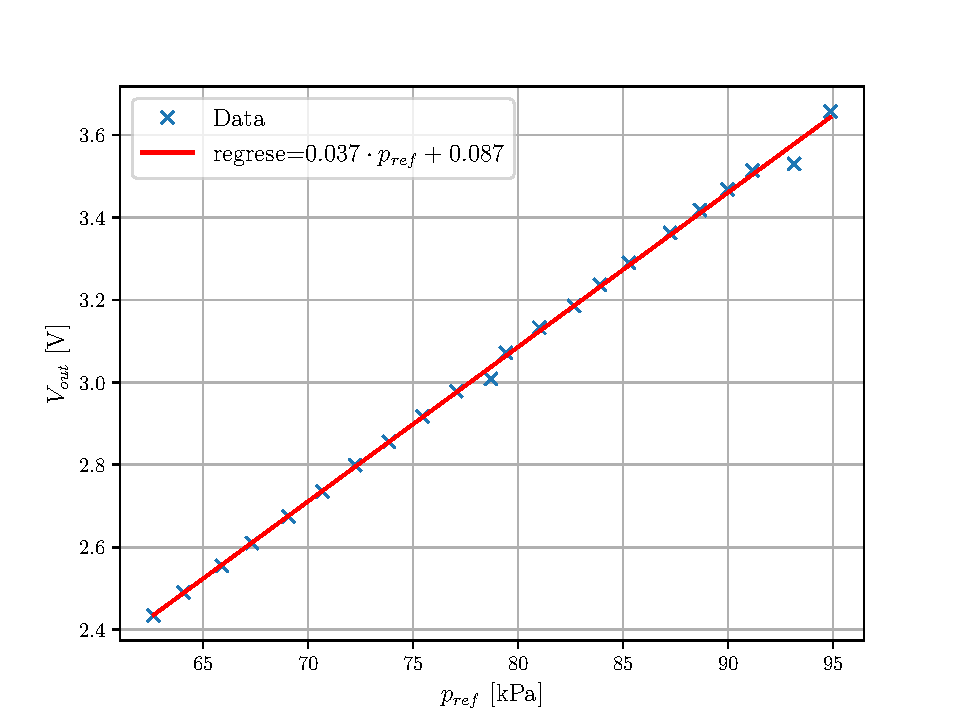
\includegraphics[width=0.8\textwidth]{img/graf-1.pdf}
            \caption{Závislost výstupního napětí na referenčním tlaku.}
            \label{fig:img/graf-1}
        \end{figure}

        \begin{figure}[h!]
            \centering
            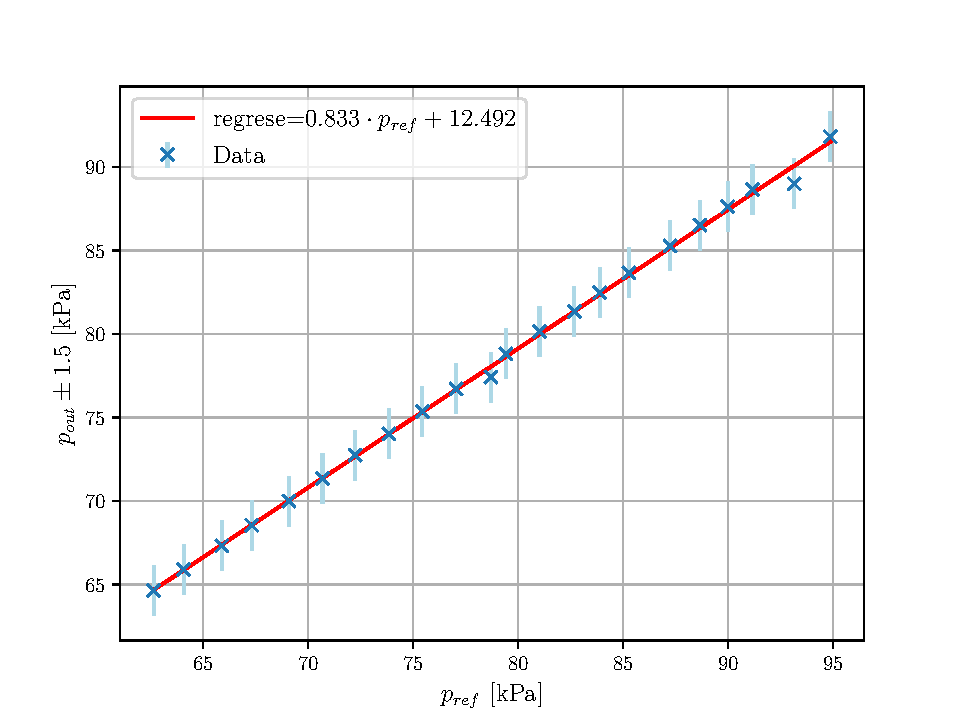
\includegraphics[width=0.8\textwidth]{img/graf-2.pdf}
            \caption{Závislost vypočítaného tlaku na referenčním tlaku.}
            \label{fig:img/graf-2}
        \end{figure}

        \begin{figure}[h!]
            \centering
            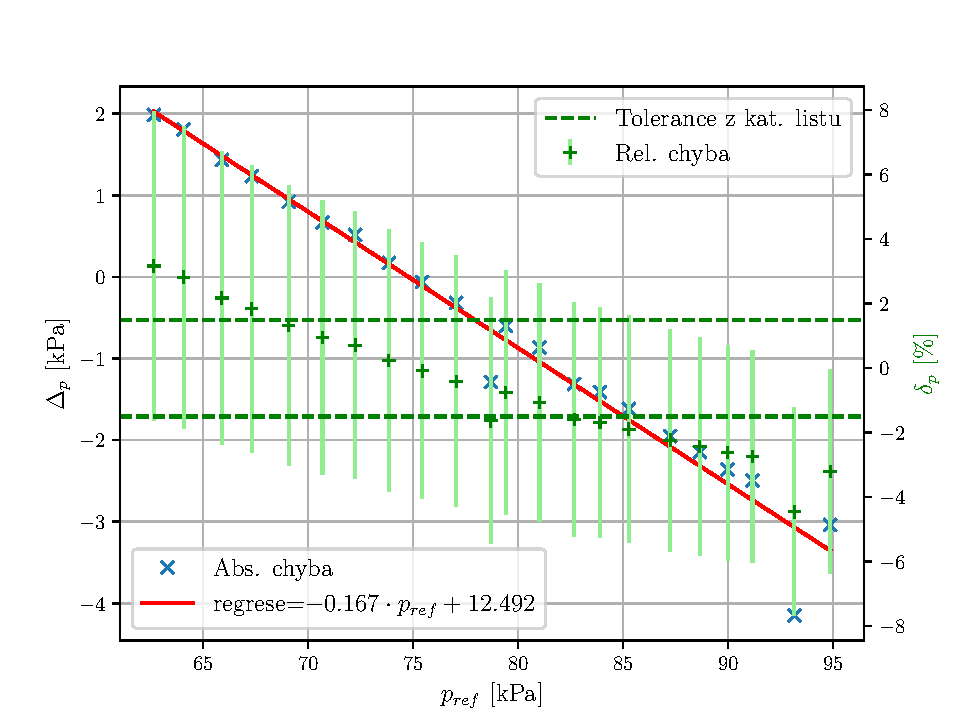
\includegraphics[width=0.8\textwidth]{img/graf-3.pdf}
            \caption{Závislost chyby měření na referenčním tlaku.}
            \label{fig:img/graf-3}
        \end{figure}
        
        \clearpage
        \section*{Závěr}
            V této úloze jsme pracovali s čidlem tlaku MPX4115A a prováděli jsme referenční měření přístrojem ALMEMO na základě kterého jsme vytvořili kalibrační křivku. 
            
            Výrobce uvádí vzorec pro výpočet tlaku z výstupního napětí senzoru s maximální abs. chybou \qty{1.5}{kPa} a garantuje také maximální relativní chybu \qty{1.5}{\percent} napříč měřícím rozsahem 15 až \qty{115}{kPa}. Přesnost přístoje ALMEMO je nám neznámá, proto ho budeme v tuto chvíli považovat za dokonale přesný a poslouží jako přístroj referenční. 

            Z hodnot získaných ze senzoru jsme stanovili absolutní chybu vůči přístroji ALMEMO a z ní pak také relativní chybu, pokud vezmeme v potaz absolutní chybu danou katalogovým listem, ověřili jsme, že se všechny měřené hodnoty nacházejí v intervalu \(\pm \qty{1.5}{\percent}\) definovaném výrobcem.

            Pro stanovení přesnosti provedené kalibrace by bylo potřeba měření opakovat vícekrát (pro stanovení stability měřené hodnoty) a také definovat přesnost přístroje ALMEMO.
\end{document}
